
\chapter{Diskrete Standortplanung} % (fold)
\label{cha:diskrete_standortplanung}

  \section{Klassifikation diskreter Standortprobleme} % (fold)
  \label{sec:klassifikation_diskreter_standortprobleme}

    \par \textbf{Planungshorizont}
    \par Anzahl der Zeitperioden (z. B. Monate, Jahre) im Planungszeitraum.
    \begin{itemize}
      \item Statische (Ein-Perioden) Modelle\\
      Standortentscheidungen werden zu Beginn des Planungshorizontes getroffen
      \item Dynamische (Mehr-Perioden) Modelle\\
      Entscheide wo und wann, d. h. in welcher Periode, Einrichtungen platziert werden.
    \end{itemize}

    \par \textbf{Einrichtungstypen}
    \par Unterscheide verschiedene Ausprägungen von Einrichtungen,

    \par \textbf{Produktaggregation}
    \par Ist nur ein Produkt oder sind mehrere Produkte mit unterschiedlichen Charakteristiken zu planen?

    \par \textbf{Stufigkeit}
    \par Anzahl der Stufen des Distributionsnetzwerks.
    \begin{itemize}
      \item Einstufige Modelle\\
      Güterverteilung über eine Transportstufe (z. B. Lager$\rightarrow$Händler). Standortentscheidung nur auf einer Ebene (z. B. Lager).
      \item Mehrstufige (hierarchische) Modelle\\
      Güterverteilung über mehrere Transportstufen (z. B. Werk$\rightarrow$Lager$\rightarrow$Händler).
    \end{itemize}

    \par \textbf{Interaktion}
    \par Interaktion zwischen Einrichtungen desselben Typs möglich, z. B. Transporte zwischen Warenhäusern.

    \par \textbf{Unsicherheit}
    \begin{itemize}
      \item Deterministische Modelle\\
      alle Daten und Parameter sind vollständig bekannt
      \item Probabilistische (stochastische) Modelle\\
      manche Daten und Parameter sind unsicher
    \end{itemize}

    \par \textbf{Flussrichtung}
    \begin{itemize}
      \item Distributionslogistik\\
      Waren fließen von Werken/Lieferanten zu den Lagern/Kunden
      \item Entsorgungslogistik (Reverse Logistics)\\
      Waren fließen von Kunden zu Recyclinganlagen, Deponien
    \end{itemize}

    \par \textbf{Kapazitätsrestriktionen}
    \par Beschränken die Mengen, welche produziert, transportiert, umgeschlagen etc. werden können.

    \par \textbf{Transportmodus}
    \begin{itemize}
      \item Touren-Belieferungen\\ 
      Auslieferungen von einer übergeordneten Einrichtung zu untergeordneten Einrichtungen (oder umgekehrt) werden zu Touren gebündelt.
      \item Direkt-Belieferungen\\ 
      Auslieferungen von übergeordneten zu untergeordneten Ebenen geschehen direkt und ohne Umwege.
    \end{itemize}
    
    \par \textbf{}


  
  % section klassifikation_diskreter_standortprobleme (end)

  \section{Das Warehouse Location Problem (WLP)} % (fold)
  \label{sec:das_warehouse_location_problem_}

    \par Auch als \textbf{Uncapacitated Facility Location Problem (UFLP)} oder \textbf{Simple Plant Location Problem (SPLP)} bekannt.

    \par \textbf{Modell-Annahmen}
    \begin{itemize}
      \item statisch, einstufig, unkapazitiert, deterministisch
      \item ein Produkt, Direkt-Belieferung, ein Einrichtungstyp, keine Interaktion
    \end{itemize}

    \par \textbf{Gegeben}
    \begin{itemize}
      \item Menge von Kunden $I = \{1, \dots, n\}$ mit Bedarfen $b_i, i = 1, \dots, n$
      \item Menge potentieller Standorte $J = \{1, \dots, m\}$ für neue Einrichtungen
      \item Kosten $t_{ij}$ für den Transport einer Mengeneinheit vom potentiellen Standort $j \in J$ zu einem Kunden $i \in I$.
      $\rightarrow$ Gesamtkosten zur Belieferung des Kunden $i$ vom Standort $j$: $c_{ij} = b_i \cdot t_{ij}$ \\$\rightarrow$ Kostenmatrix $C = (c_{ij})_{i = 1, \dots, n, j = 1, \dots, m}$
      \item Fixkosten $f_j$ für die Errichtung einer neuen Einrichtung am Standort $j$.
    \end{itemize}

    \par \textbf{Entscheidungen}
    \begin{itemize}
      \item Anzahl neuer Einrichtungen
      \item Standorte neuer Einrichtungen
      \item Zuordnung von Kunden zu neuen Einrichtungen
    \end{itemize}


    \subsection{Modellierug} % (fold)
    \label{sub:modellierug}

      \par \textbf{Standortentscheidung}
      $$
        y_j = 
        \begin{cases}
          1 & \text{falls am potentiellen Standort } j \text{ eine neue Einrichtung platziert wird}, j \in J\\
          0 & \text{sonst}
        \end{cases} 
      $$

      \par \textbf{Zuordnungsentscheidung}
    
      $$
        x_{ij} = 
        \begin{cases}
          1 & \text{falls Kunde i einer neuen Einrichtung am Standort } j \text{ zugeordnet wird}, i \in I, j \in J\\
          0 & \text{sonst}
        \end{cases} 
      $$

      \par \textbf{Mathematisches Modell}

      \begin{equation}
        \begin{aligned}
          & \underset{}{\text{min}}
          && \sum_{i=1}^{n}\sum_{j=1}^{m}c_{ij}x_{ij} + \sum_{j=1}^{m}f_ky_{j}\\
          % & & e - (s + re) \\
          & \text{u.d.N}
          & & \sum_{j=1}^{m}x_{ij}=1, \forall i \qquad  (\text{Jeder Kunde } i \text{ wird genau einer neuen Einrichtung an einem Standort } j \text{ zugeordnet})\\ 
          & & & x_{ij} \leq y_j, \forall i, \forall j \quad \text{(Kunde } i \text{ darf nur dann Standort } j \text{ zugeordnet werden, wenn an } j \text{ eine Einrichtung platziert)}\\ 
          & & & x_{ij} \geq 0, y_j \in \{0,1\}, \forall i, \forall j \\
        \end{aligned}
      \end{equation}

    % subsection modellierug (end)

    \subsection{Heuristiken} % (fold)
    \label{sub:heuristiken}

      Methoden zur Bestimmung einer heuristischen Lösung $X_H$ für ein Problem.

      (Finden nicht notwendigerweise eine optimale Lösung.)

      \par \textbf{Güte einer heuristischen Lösung $X_H$}:Relative Abweichung in Prozent

      $$
        RPD(X_H, X^*) = \frac{f(X_H) - f(X^*)}{f(X^*)} * 100\% \leq \frac{f(X_H) - LB}{LB}
      $$

      \par Es gibt zwei Klassen von Standort-Zuordnungs-Heuristiken:
      \begin{itemize}
        \item Konstruktionsheuristiken: Bestimmen „aus dem Nichts heraus“ eine Lösung des Problems. 
        \begin{itemize}
          \item Greedy (ADD-Heuristik)
          \item Stingy (DROP-Heuristik)
        \end{itemize}
        \item Verbesserungsheuristiken: Versuchen eine bereits vorhandene Lösung zu verbessern.
        \begin{itemize}
          \item Interchange (ADD\&DROP-Heuristik)
          \item Metaheuristiken: Variable Neighborhood/Tabu Search, Genetic Algorithms
        \end{itemize}
      \end{itemize}

      \subsubsection{Greedy-Heuristik}

        \begin{algorithm}[H]
          \begin{algorithmic}[1]
            \caption{Greedy-Heuristik}
            \State Init: $X^0:=\varnothing, J':= J, l:=1$. Berechne $u_i^0 = \underset{j=1,\dots, m}{\text{max}}c_{ij}, F(X^0)=\sum_{i=1}^{n}u_i^0$
            \While{($J \neq \varnothing$)}
              \State Berechne $\vartriangle_j^l = \sum_{i=1}^{n}\text{max}\{0, u_i^{l-1} -c_{ij}\}$ und $\omega_j^l = \vartriangle_j^l - f_j = \sum_{i=1}^{n}\text{max}\{0, u_i^{l-1} -c_{ij}\} - f_j, \forall j \in J'$
              \State Bestimme potentiellen Standort $j \in J'$ mit $$\tilde{\omega}_j^l = \underset{k \in J'}{\text{max}}\{\omega_k^l: \omega_k^l > 0\}$$
              \State $X^l := X^{l-1} \cup \{j\}, J':= J'\setminus\{j\}, F(x^l) = F(X^{l-1}) - \tilde{\omega}_j^l$
              \If{($\omega_h^l \leq 0, h \in J'$)}
                \State $J:= J' \setminus \{h\}$
              \EndIf
              \State Aktualisiere geringste Kosten für alle Kunden $i$: $u_i^l = \text{min}\{c_{ij} | j \in X^l\}$
              \State $l:= l+1$
            \EndWhile
            \end{algorithmic}
          \textbf{Output:eine heuristische Lösung des Problems $X^{l-1}$} 
        \end{algorithm}

        % \begin{note}
          
        % \end{note}

        \begin{exmp}
          
        \end{exmp}

        \begin{figure}[H]
          \centering
          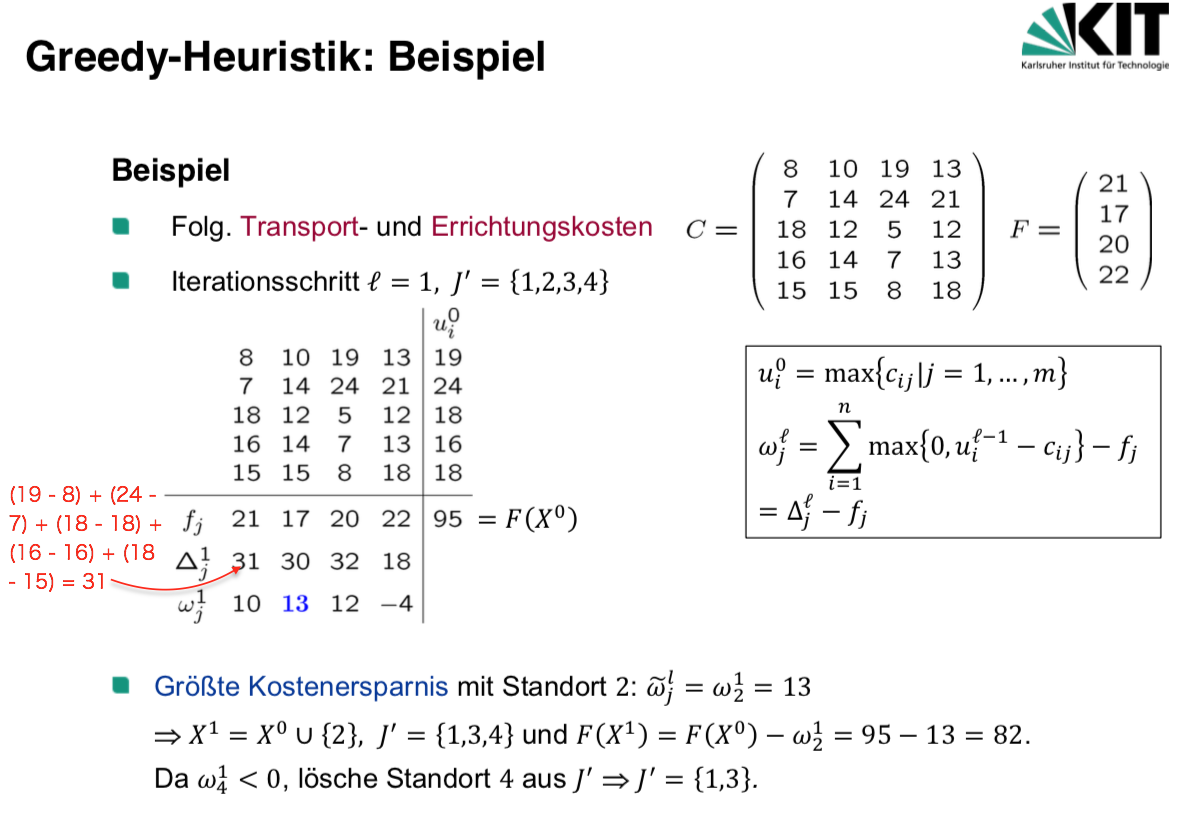
\includegraphics[width=0.95\textwidth]{Images/Greedy_Heuristik_Bsp(1).png}
          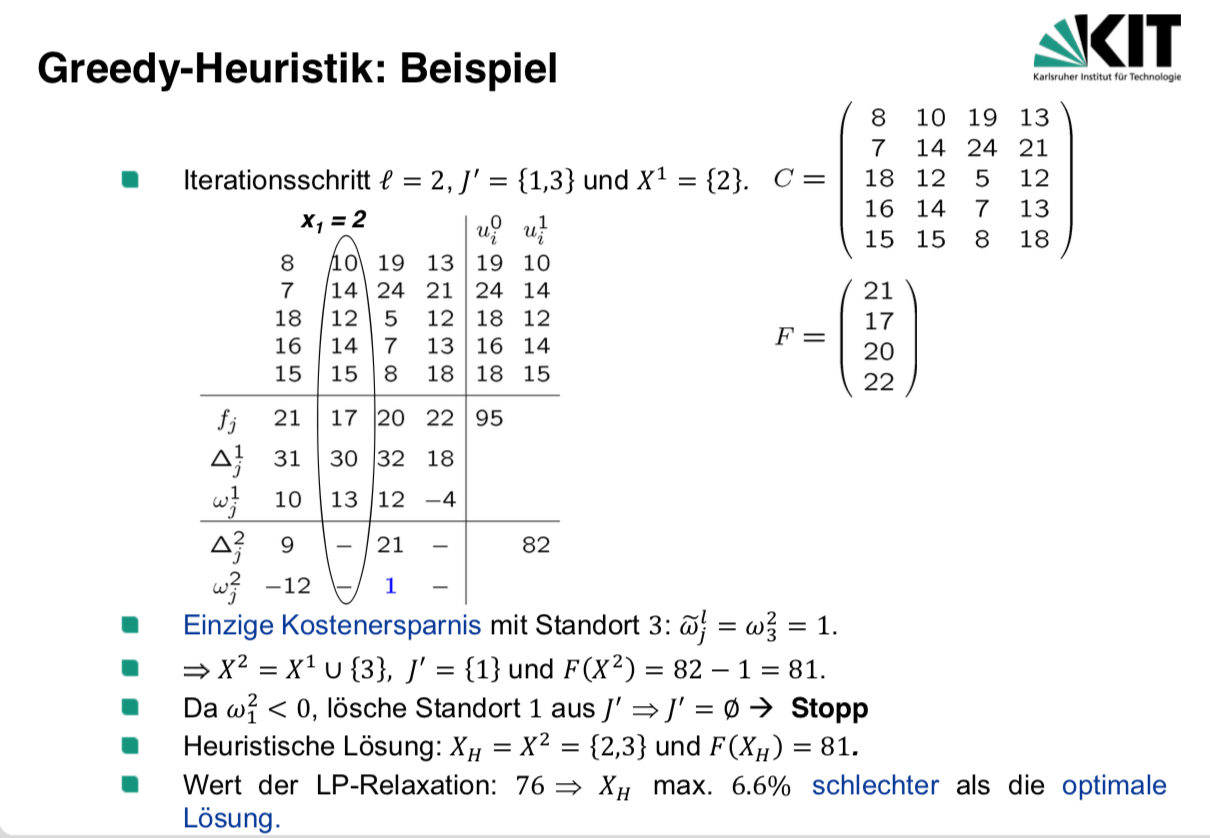
\includegraphics[width=0.95\textwidth]{Images/Greedy_Heuristik_Bsp(2).png}
          \caption{Greedy Heuristik Bsp}
          \label{fig:Greedy_Heuristik_Bsp}
        \end{figure}

        \begin{exmp}
          \color{blue}{Aufgabe 14}
        \end{exmp}

      \subsubsection{Interchange-Heuristik}

    % subsection heuristiken (end)

    \subsection{Das DUALOC-Verfahren} % (fold)
    \label{sub:das_dualoc_verfahren}

      \begin{figure}[H]
        \centering
        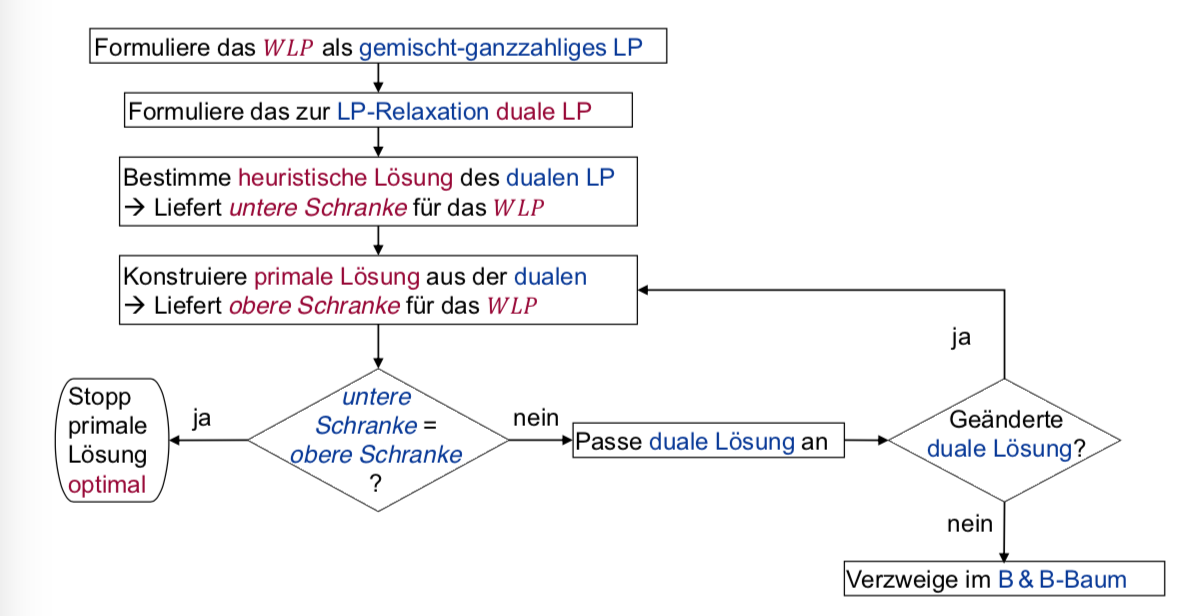
\includegraphics[width=0.95\textwidth]{Images/DUALOC_Verfahren.png}
        \caption{DUALOC-Verfahren}
        \label{fig:DUALOC_Verfahren}
      \end{figure}

      \begin{exmp}
          \color{blue}{Aufgabe 15, 16}
        \end{exmp}

      \par \textbf{1. WLP als gemischt-ganzzahliges lineares Programm}

      \begin{equation}
        \begin{aligned}
          & \underset{}{\text{min}}
          && \sum_{i=1}^{n}\sum_{j=1}^{m}c_{ij}x_{ij} + \sum_{j=1}^{m}f_jy_{j}\\
          % & & e - (s + re) \\
          & \text{u.d.N}
          & & \sum_{j=1}^{m}x_{ij}=1, \forall i \\
          & & & x_{ij} \leq y_j, \forall i, \forall j \\ 
          & & & x_{ij} \geq 0, y_j \in \{0,1\}, \forall i, \forall j \\
        \end{aligned}
      \end{equation}

      \par \textbf{LP-Relaxation (LP)} des gemischt-ganzzahligen linearen Programms für das WLP

      \begin{equation}
        \begin{aligned}
          & \underset{}{\text{min}}
          && \sum_{i=1}^{n}\sum_{j=1}^{m}c_{ij}x_{ij} + \sum_{j=1}^{m}f_ky_{j}\\
          % & & e - (s + re) \\
          & \text{u.d.N}
          & & \sum_{j=1}^{m}x_{ij}=1, \forall i \\
          & & & x_{ij} \leq y_j, \forall i, \forall j \\ 
          & & & x_{ij} \geq 0, y_j \geq 0, \forall i, \forall j \\
        \end{aligned}
      \end{equation}

      \par \textbf{2. duale lineare Programm (DP)} ) mit den Dual-Variablen $v_i$ und $w_{ij}$ 

      \begin{equation}
        \begin{aligned}
          & D(v, w) = \text{max}
          && \sum_{i=1}^{n}v_i\\
          % & & e - (s + re) \\
          & \text{u.d.N}
          & & \sum_{i=1}^{n}w_{ij} \leq f_j, \forall j \\
          & & & v_i - w_{ij} \leq c_{ij}, \forall i, \forall j \\
          & & & v_i \lessgtr 0, \forall i\\
          & & & w_{ij} \geq 0, \forall i, \forall j
        \end{aligned}
      \end{equation}

      \par \textbf{Reduziertes duales LP (RDP)}

      \begin{equation}
        \begin{aligned}
          & D(v, w) = \text{max}
          && \sum_{i=1}^{n}v_i\\
          % & & e - (s + re) \\
          & \text{u.d.N}
          & & \sum_{i=1}^{n}max\{0, v_i- c_{ij}\} \leq f_j, \forall j \\
          % & & & v_i - w_{ij} \leq c_{ij}, \forall i, \forall j \\
          & & & v_i \lessgtr 0, y_j \geq 0, \forall i
          % & & & w_{ij} \geq 0, \forall i, \forall j
        \end{aligned}
      \end{equation}

      \par 3. Löse das (RDP) mit dem \textbf{Dual Ascent-Verfahren} und erhalte eine heuristische Lösung von (DP). $\rightarrow$ liefert die untere Schranke für das (WLP).

      \subsection{Dual Ascent-Verfahren} % (fold)
      \label{sub:dual_ascent_verfahren}

        \par \textbf{Idee/Vorgehensweise}
        \par Erhöhe, ausgehend von einer Startlösung $v$, reihum jedes $v_i$ solange um einen kleinen Wert, bis keines mehr erhöht werden kann.

        \par Definiere:
        \begin{itemize}
          \item $J_i := \{j \in J | v_i \geq c_{ij}\}$
          \item $s_j := f_j - \sum_{i = 1}^{n}max\{0, v_i - c_{ij}\}, \forall j in J$
          \item $k(i) := min\{k|c_i^k \geq v_i\}$
        \end{itemize}

        \begin{algorithm}[H]
          \begin{algorithmic}[1]
            \caption{Dual Ascent-Verfahren}
            \State Init:
            \State Sortiere die Kostenelement $c_{ij}$ jedes Kunden $i \in I$ nach monoton zunehmenden Werten und bezeichne sie mit $c_i^k$: $c_i^1 \leq c_i^2 \leq \dots \leq c_i^m \leq c_i^{m+1}:= \infty$
            \State $I':= I, v_i := c_i^1$ für $\forall i \in I$
            \State Berechne $J_i := \{j \in J | v_i \geq c_{ij}\}, \forall i \in I$ und  $s_j := f_j - \sum_{i = 1}^{n}max\{0, v_i - c_{ij}\}, \forall j \in J$
            \State Bestimme $k(i) := min\{k|c_i^k \geq v_i\}, \forall i \in I$
            \If{($v_i = c_i^{k(i)}$)} 
              \State $k(i) := k(i) + 1$
            \EndIf
            \While{($I' \neq \varnothing$)}
              \State Für $\forall i \in I'$: Bestimme $\vartriangle_i := min\{s_j|j \in J_i\}$
              \If{($\vartriangle_i = 0$)}
                \State $I':=I' \setminus \{i\}$
                \State Wähle das nächste $i \in I'$
              \Else
                \State Setze $\vartriangle = min\{\vartriangle_i, c_i^{k(i)} - v_i\}$
                \If{($\vartriangle = \vartriangle_i$)}
                  \State $I' := I' \setminus \{i\}$
                \Else 
                  \State $k(i) := k(i) + 1$
                \EndIf
                \State Setze $v_i := v_i + \vartriangle$ 
                \State Für $\forall j \in J_i$, setze $s_j := s_j - \vartriangle$
                \State Aktualisiere $J_i$
              \EndIf
            \EndWhile
            \end{algorithmic}
          \textbf{Output:eine heuristische Lösung von (RDP) (Untere Schranke für das (WLP))} 
        \end{algorithm}

        \begin{exmp}
          
        \end{exmp}
      
        \begin{figure}[H]
          \centering
          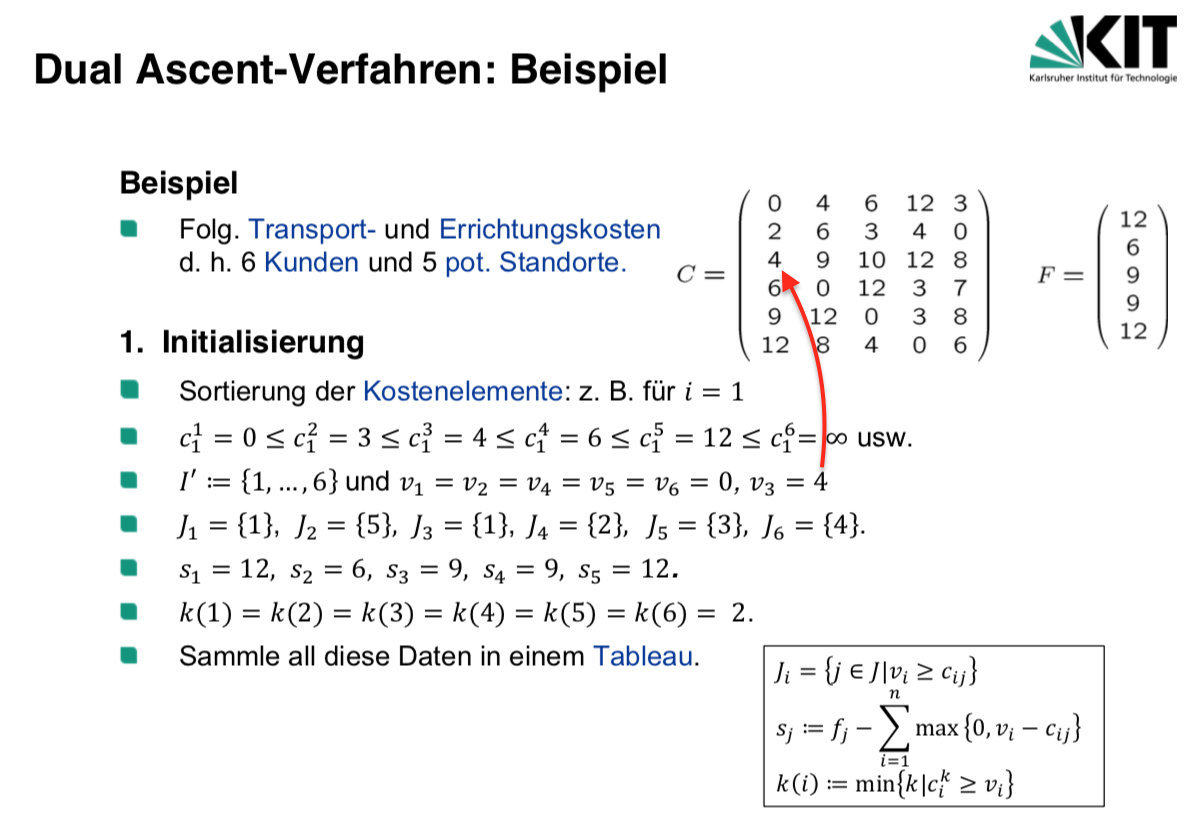
\includegraphics[width=0.95\textwidth]{Images/Dual_Ascent_Verfahrten_Bsp(1).png}
          \caption{Dual Ascent-Verfahren Bsp}
          \label{fig:dual_ascent_verfahren_bsp}
        \end{figure}

        \begin{figure}[H]
          \centering
          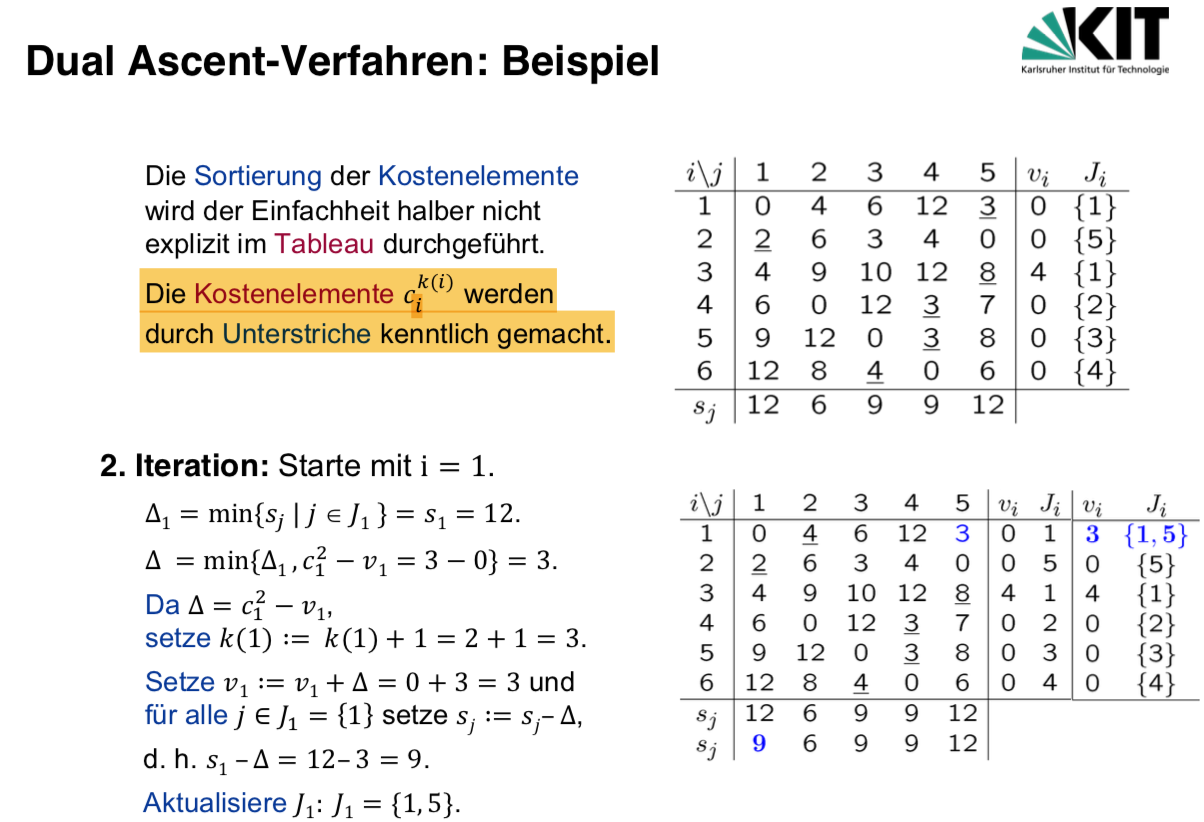
\includegraphics[width=0.95\textwidth]{Images/Dual_Ascent_Verfahrten_Bsp(2).png}
          \caption{Dual Ascent-Verfahren Bsp}
          \label{fig:dual_ascent_verfahren_bsp}
        \end{figure}

        \begin{figure}[H]
          \centering
          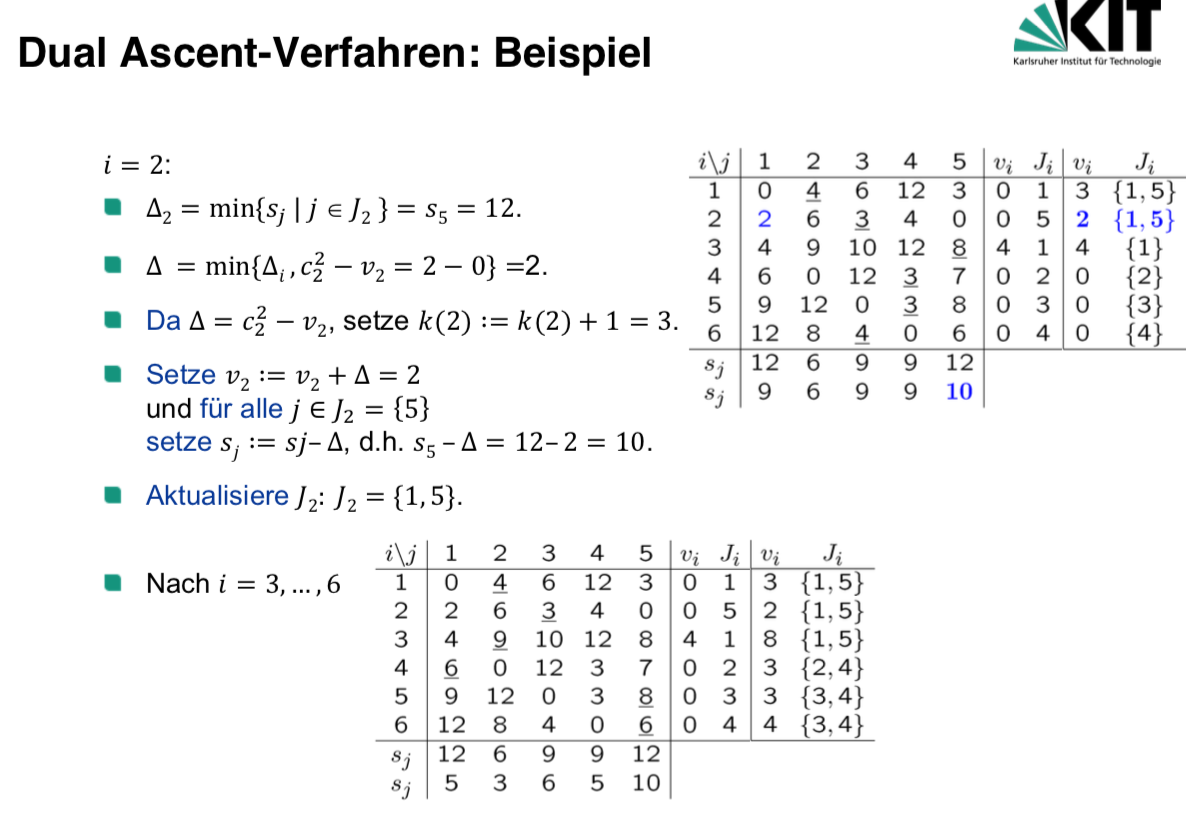
\includegraphics[width=0.95\textwidth]{Images/Dual_Ascent_Verfahrten_Bsp(3).png}
          \caption{Dual Ascent-Verfahren Bsp}
          \label{fig:dual_ascent_verfahren_bsp}
        \end{figure}

        \begin{figure}[H]
          \centering
          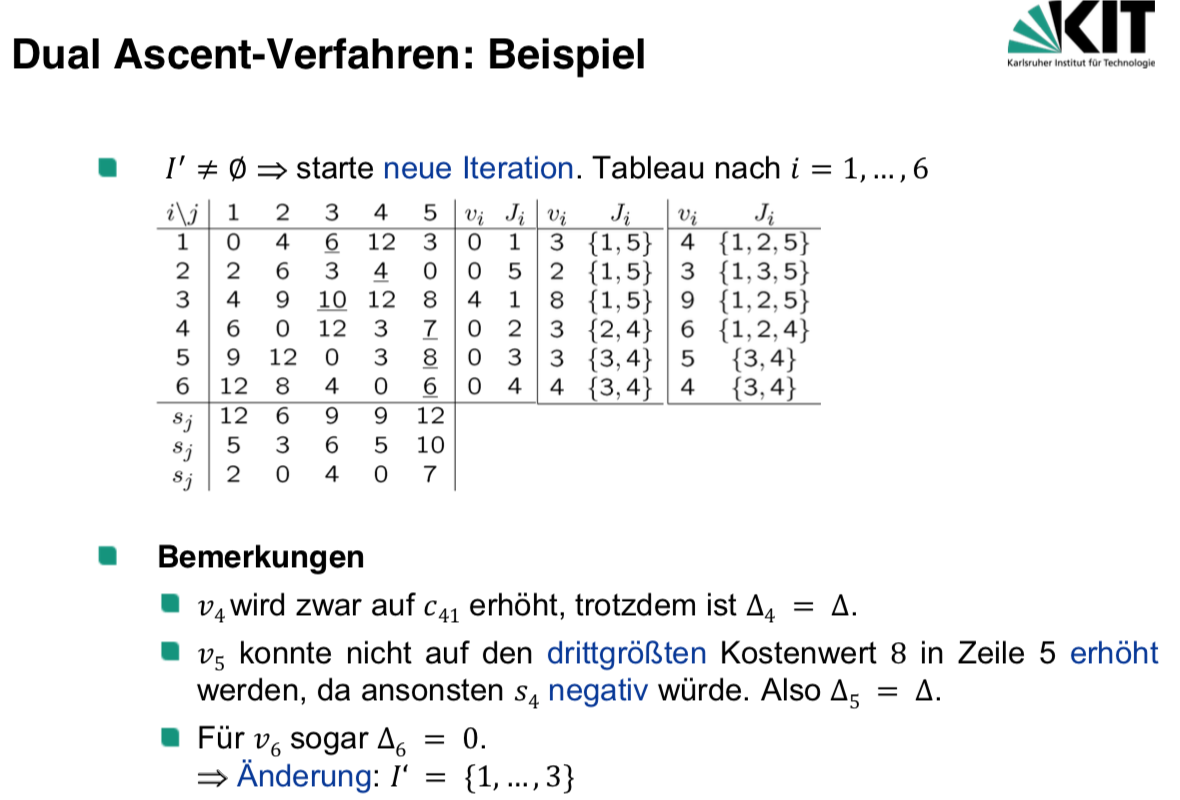
\includegraphics[width=0.95\textwidth]{Images/Dual_Ascent_Verfahrten_Bsp(4).png}
          \caption{Dual Ascent-Verfahren Bsp}
          \label{fig:dual_ascent_verfahren_bsp}
        \end{figure}

        \begin{figure}[H]
          \centering
          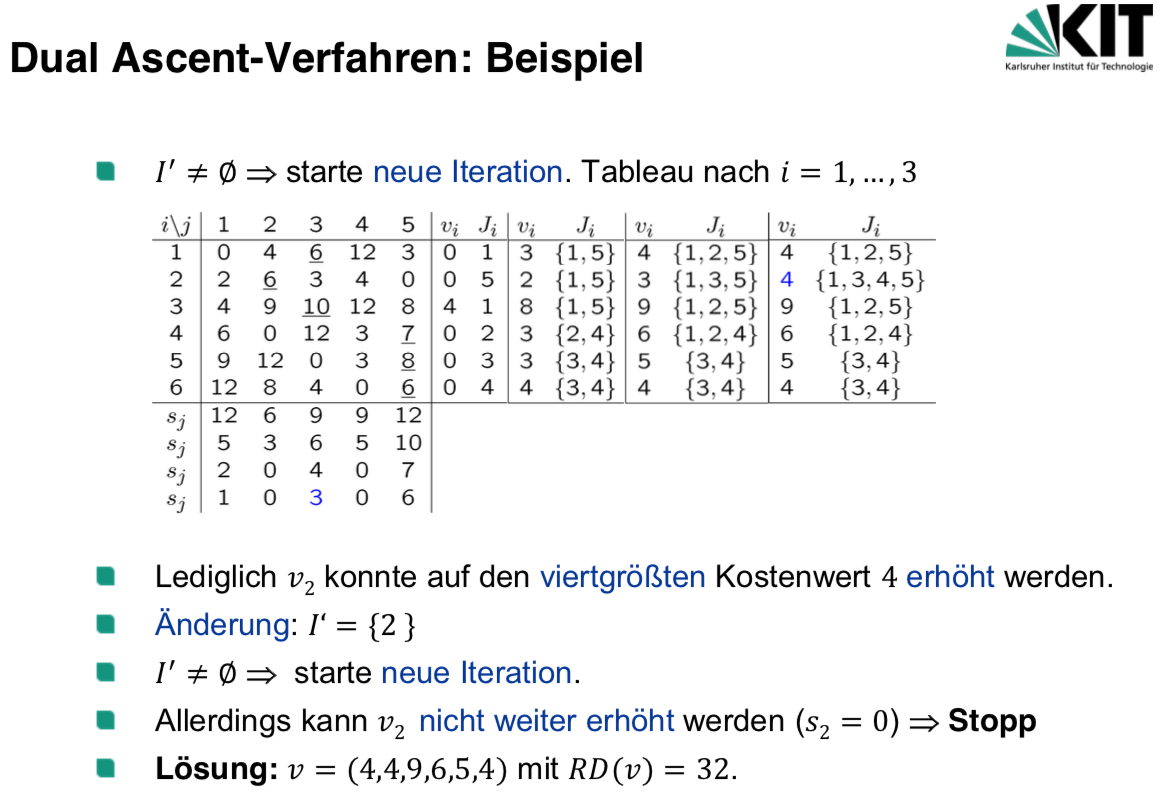
\includegraphics[width=0.95\textwidth]{Images/Dual_Ascent_Verfahrten_Bsp(5).png}
          \caption{Dual Ascent-Verfahren Bsp}
          \label{fig:dual_ascent_verfahren_bsp}
        \end{figure}
      % subsection dual_ascent_verfahren (end)


      \par 4. Konstruiere primär Lösung ausgehend von einer zulässinge Lösung $v$ von (RDP) mit \textbf{Konstruktionsheuristik} $\rightarrow$ liefert die obere Schranke für das (WLP)

      \subsection{Konstruktionsheuristik} % (fold)
      \label{sub:konstruktionsheuristik}

        \begin{algorithm}[H]
          \begin{algorithmic}[1]
            \caption{Konstruktionsheuristik}
            % \State \Comment{Init:}
            \State \textbf{Init}: setze $X = \varnothing$, berechne $J^+ = \{j \in J | s_j = 0\}$
            \State \textbf{Selektion von Standorten} 
            \State Für $\forall i \in I$: 
            \If{(Es gibt für Kunde $i$ genau einen Standort $j \in J^+$ mit $c_{ij} \leq v_i$ und $j \notin X$)}
              \State Setze $X = X \cup \{j\}, y_j = 1$
            \ElsIf{(Es gibt für Kunde $i$ mehrere Standorte $j \in J^+$ mit $c_{ij} \leq v_i$, aber keines dieser $j \in X$)}
              \State setze $X = X \cup \{j^*\}, y_{j^*} = 1$ für das $j^*$ mit $c_{ij^*} = min\{c_{ij}|c_{ij} \leq v_i\}$
            \EndIf
            \State \textbf{Zuordnung}
            \State Ordne jeden Kunden $i$ dem kostengünstigsten Standort $j \in X$ zu:
            $x_{ij^*} = 1$ für das $j^*$ mit $c_{ij^*} = min\{c_{ij}|c_{ij} \leq v, j \in X\}$

            \end{algorithmic}
          \textbf{Output:primäre Lösung (obere Schranke für das (WLP))} 
        \end{algorithm}

        \begin{exmp}
          
        \end{exmp}

        \begin{figure}[H]
          \centering
          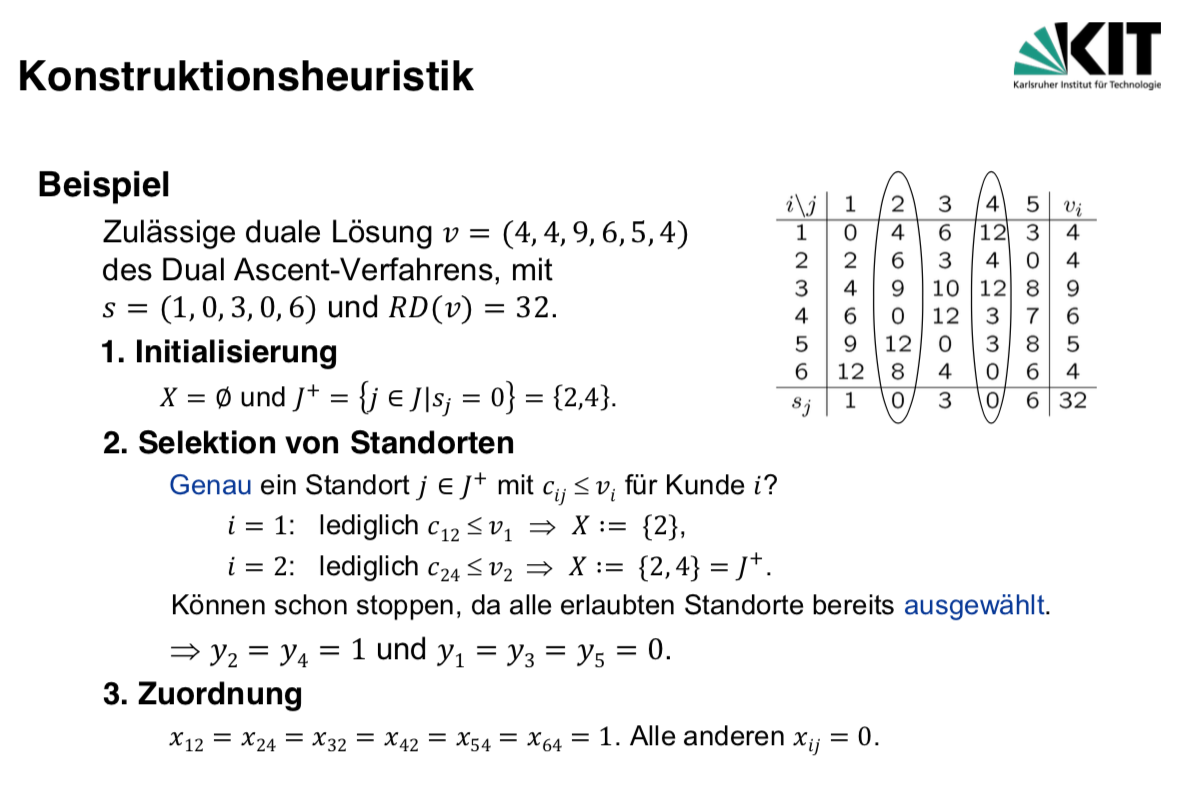
\includegraphics[width=0.95\textwidth]{Images/Konstruktionsheuristik_Bsp.png}
          \caption{Konstruktionsheuristik Bsp}
          \label{fig:Konstruktionsheuristik_Bsp}
        \end{figure}
      
      % subsection konstruktionsheuristik (end)

      \par 5. \textbf{Optimalitätsbedingungen} erfüllt?

      \begin{itemize}
        \item $s_j \geq 0 \Rightarrow y_j= 0; s_j=0 \Rightarrow y_j > 0$
        \item $v_i < c_{ij} \Rightarrow x_{ij} = 0; v_i \geq c_{ij} \Rightarrow x_{ij} \geq 0 $
        \item $v_i > c_{ij} \Rightarrow x_{ij} = y_j$
      \end{itemize}

      \par Falls die drei Bedingungen erfüllt sing $\rightarrow$ Die beide erhaltenen Lösung sind optimal
      \par Sonst $\rightarrow$ \textbf{Dual Adjustment Verfahren}, dann wieder Konstruktionsheuristik durchführen, bis die Optimalitätsbedingungen erfüllt werden. 
    

      \subsubsection{Dual Adjustment-Verfahren} % (fold)
      \label{ssub:dual_adjustment_verfahren}
      
        \par \textbf{Voraussetzung}
        \par zulässinge Lösungen $v$ von (RDP) und $(x, y)$ von (WLP).

        Definiere:
        \begin{itemize}
          \item $J_i^x := \{j \in X | v_i > c_{ij}\}$
          \item $c_{ij^*} = min\{c_{ij} | j \in J_i^x\}$
          \item $c_{ij^{**}} = min\{c_{ij} | j \in J_i^x, j \neq j^*\}$
          \item $I_j^x = \{i \in I | j \in X \text{ ist der einzige Standort mit } v_i \geq c_{ij}\}, j \in X$ 
        \end{itemize}
        
        

        \begin{algorithm}[H]
          \textbf{Input:} zulässinge Lösungen $v$ von (RDP) und $(x, y)$ von (WLP). (Nur für die Spalten mit $s_j = 0$ durchführen)
          \begin{algorithmic}[1]
            \caption{Dual Adjustment-Verfahren}
            \State \textbf{Iteration}
            \State Für $\forall i \in I$:
            \State Gilt $|J_i^x| \leq 1$ oder $I_{j^*}^x \cup I_{j**}^x = \varnothing$, so fahre mit dem nächsten $i$ fort.
            \State Bestimme das nächstkleinere $c_{ij}: \vartriangle := max\{c_{ij}|c_{ij} < v_i, j \in J\}$
            \State Setze $s_j := s_j + (v_i - \vartriangle)$ für $\forall j \in J_i^x$
            \State Setze $v_i:= \vartriangle$
            \State Führe das Dual Ascent-Verfahren nacheinander aus mit
            \begin{itemize}
              \item $I':=I_{j^*}^x \cup I_{j^{**}}^x$
              \item $I':= I' \cup \{i\}$
              \item $I':= I$
            \end{itemize}

            \end{algorithmic}
          % \textbf{Output:eine heuristische Lösung von (RDP)} 
        \end{algorithm}
      % subsubsection dual_adjustment_verfahren (end)

      \begin{exmp}
        
      \end{exmp}

      \begin{figure}[H]
        \centering
        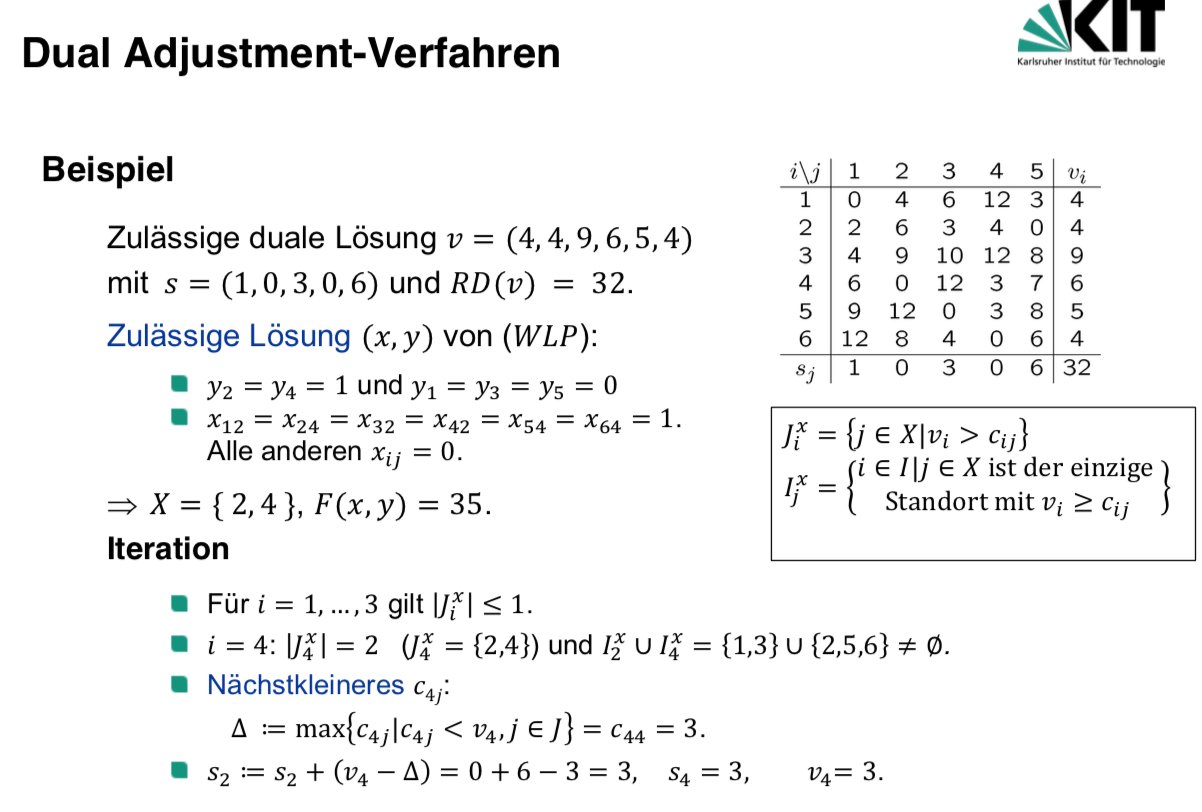
\includegraphics[width=0.95\textwidth]{Images/Dual_Adjustment_Verfahren_Bsp(1).png}
        \caption{Dual Adjustment-Verfahren Bsp}
        \label{fig:Dual_Adjustment_Verfahren}
      \end{figure}

      \begin{figure}[H]
        \centering
        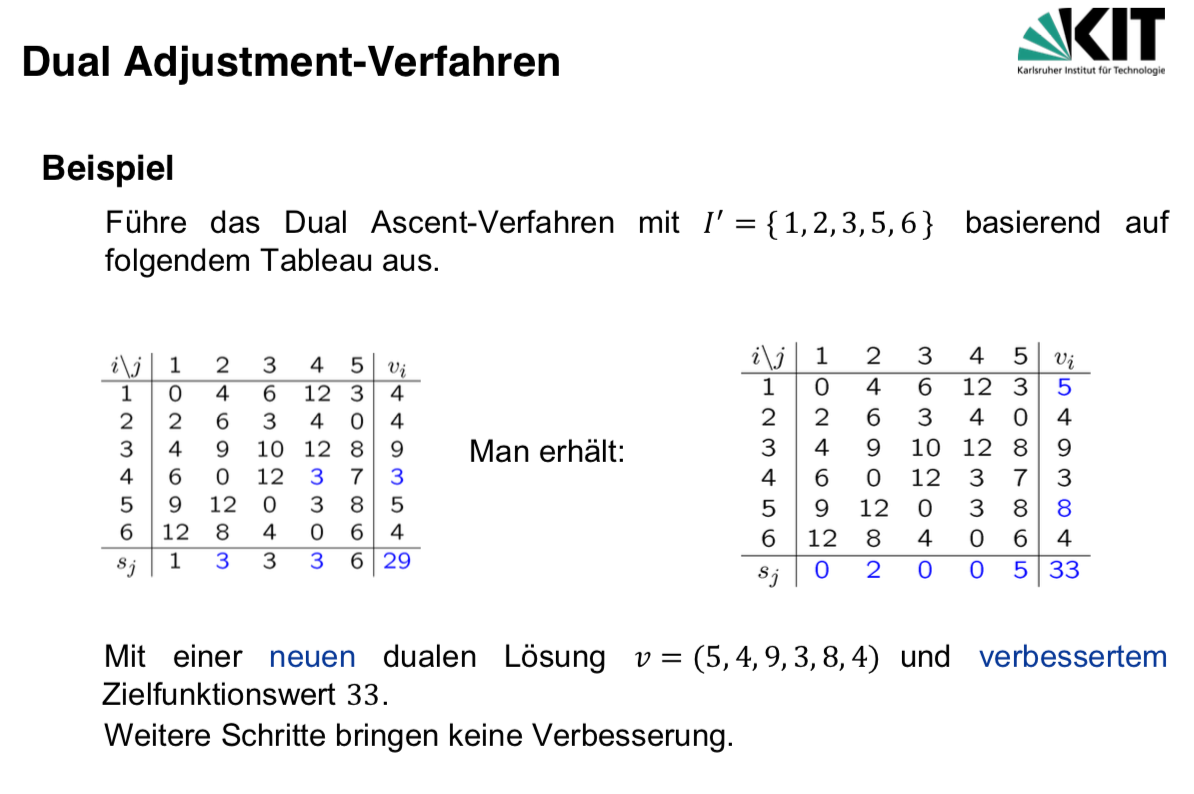
\includegraphics[width=0.95\textwidth]{Images/Dual_Adjustment_Verfahren_Bsp(2).png}
        \caption{Dual Adjustment-Verfahren Bsp}
        \label{fig:Dual_Adjustment_Verfahren}
      \end{figure}
    % subsection das_dualoc_verfahren (end)

    \begin{note}
      \begin{figure}[H]
        \centering
        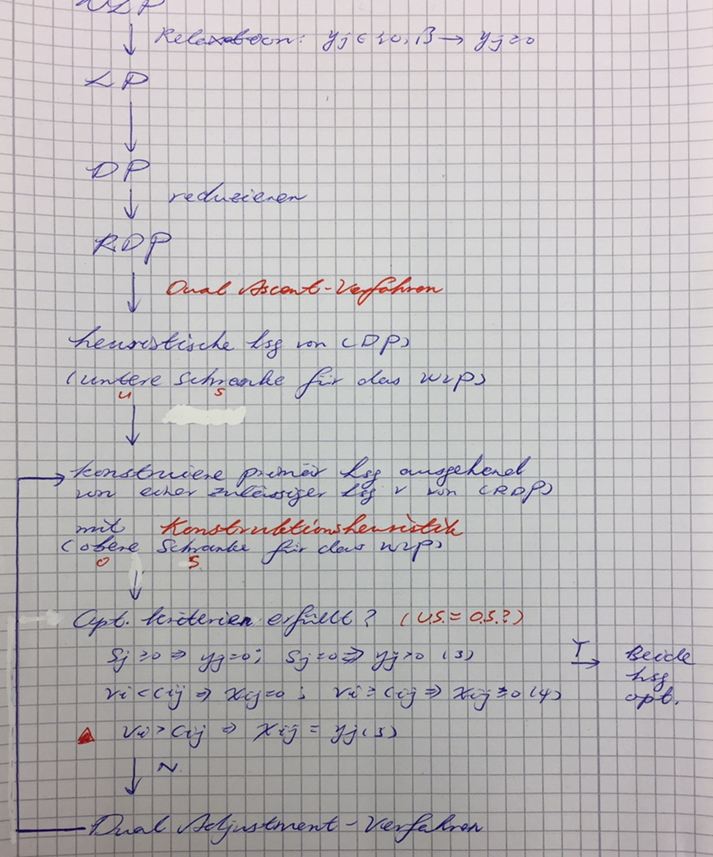
\includegraphics[width=0.95\textwidth]{Images/WLP_Zusammenfassung.JPG}
        \caption{WLP}
        \label{fig:WLP}
      \end{figure}
    \end{note}

  % section das_warehouse_location_problem_ (end)

  \section{Hub-Location-Probleme} % (fold)
  \label{sec:hub_location_probleme}
  
  % section hub_location_probleme (end)
% chapter diskrete_standortplanung (end)

    


